%%%% acra.tex

\typeout{ACRA Instructions for Authors}

% This is the instructions for authors for ACRA.
\documentclass{article}
\usepackage{acra}
% The file acra.sty is the style file for ACRA. 
% The file named.sty contains macros for named citations as produced 
% by named.bst.

% The preparation of these files was supported by Schlumberger Palo Alto
% Research, AT\&T Bell Laboratories, and Morgan Kaufmann Publishers.
% Shirley Jowell, of Morgan Kaufmann Publishers, and Peter F.
% Patel-Schneider, of AT\&T Bell Laboratories collaborated on their
% preparation. 

% These instructions can be modified and used in other conferences as long
% as credit to the authors and supporting agencies is retained, this notice
% is not changed, and further modification or reuse is not restricted.
% Neither Shirley Jowell nor Peter F. Patel-Schneider can be listed as
% contacts for providing assistance without their prior permission.

% To use for other conferences, change references to files and the
% conference appropriate and use other authors, contacts, publishers, and
% organizations.
% Also change the deadline and address for returning papers and the length and
% page charge instructions.
% Put where the files are available in the appropriate places.
\usepackage[pdftex]{graphicx}
%\usepackage{epstopdf}
% declare the path(s) where your graphic files are
\graphicspath{{../resources/}{../resources/tmp/}}
% and their extensions so you won't have to specify these with
% every instance of \includegraphics
\DeclareGraphicsExtensions{.pdf,.svg,.png}


\title{Middleware for Parallelization of Multiplayer Simulation}
\author{Peter Böhm \\ ACME University, Australia \\ 
peter@nextlogic.biz}

\begin{document}

\maketitle

\begin{abstract}
Computer simulations have become the standard for modeling of behavior of various natural systems. The more complex the model, the more sophisticated and more expansive hardware is required to run the simulation including multiple CPUs and GPUs. To achieve a realistic model, the simulation needs to be run on a high fidelity simulator like Microsoft's AirSim. Once the data has been generated, they need to be analyzed and the results visualized. The simulations often generate considerable amount of data about the simulated processes such as positions, velocities, rotations, collisions, environmental conditions, etc. During the simulation, these data need to be available to the solver for decision making calculations and possibly a progress visualizer. The data also need to be persisted for future analysis. When modeling interaction between multiple agents, the control and tracking of agents needs to be parallelized to allow for asynchronous operation and communication. The updates cannot happen in a single threaded control loop because that would introduce undesirable delays and move dependencies. The amount of work needed to create this supporting infrastructure is substantial and needs to be repeated or duplicated for every project. A middleware encapsulating these auxiliary services is presented.
\end{abstract}

\section{Introduction}

\emph{Something about various uses of UAVs and importance of determination of the right strategy. Probably mention differential games as a theoretical framework and a couple of sentences about how it uses diff equations to describe the state. The simulation can be used to confirm the results in a realistic setting but also to train the agents, e.g. using RL. }

\emph{Couple of sentences about simulators, how they are important because the realistically model the environment and it's one less very messy thing to worry about. Briefly discuss some of the available sims, their strengths and weaknesses?}
To provide a realistic real-world model is a non-trivial task. This is especially important, if the simulator is used for training of the agents that will eventually operate in the real world. In such cases, the agents need to rely on inputs that are also available in real world such as depth view, segmentation view or the FPV (first-person view). In this case it may be important to model real-world complex objects such as trees, roads, lakes, electric poles and houses along with rendering that includes finer deteails such as soft shadows, specular reflections, diffused inter-reflections and so on. \cite{shah2018airsim}
\emph{maybe an image with the 3 views}

\emph{More details about AirSim - something like the conclusion from the MS paper. How it provides actual location but also sensors}

\subsection{Background} 
Because the simulator provides a realistic world-like model, it also needs to be interacted with in a realistic way. One of the main differences when compared to the low or mid fidelity simulators, such as OpenAI Gym, is absence of a turn by turn event loop.
E.g., the Mountain Car problem in OpenAI Gym simulates effects gravity and inertia, however, after every action taken by the agent, the time is suspended. The agent can take as long as it needs to calculate the next action. At that point, the time and physics starts moving again and the car moves without any loss of inertia or speed.
\begin{figure}
	\centering
	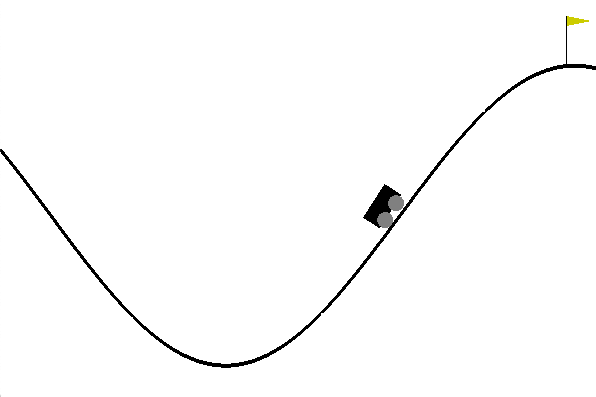
\includegraphics[width=7cm]{mountain-car}
	\caption{Mountain car problem in the OpenAI Gym. The car can be suspended and resumed without any loss of momentum.}\label{fig:mountain-car}
\end{figure}

In a high fidelity simulator, the situation is different. The agents receive commands, however, the time and the underlying physics do not stop in between the commands. As such it is important that the tasks that can run in parallel, such as location tracking and controlling of the agent are parallelized. This is especially important in multi-agent simulations, where the forced sequence and the delay between actions of the agents can have material impact on the progress and results of the simulation. Usually, this would involve sampling of the environment state (e.g. location updates, sensor measurements, image from the camera, etc.), processing this input (e.g. calculation of relative distances, LIDAR points analysis), calculation of the new direction/speed and sending of the commands to the agents.

\subsection{Design}

\emph{Example of a naive python program working with AirSim - sending instructions and receiving state updates. First show figure with only the 2 processes and then add on everything else necessary and show how it becomes entangled. Then split it up into the solver, persistence, visualization, etc. all connected by the middleware. }

\section{Programming Model}
Need for new programming model (something like Akka Docs intro).
Building blocks - actors, messages, streams (graph processing), Kafka?
Explain individual components of the simulator - simulator, trackers (camera/lidar tracking???), relative position (belongs to the solver), players, referee. How they pass messages, how they send updates to Kafka and receive directions from Kafka.
Kafka... simplify dependencies between services, reduce data loss when a service crashes, simplicity of one "API" for communication.

\begin{figure}
	\centering
	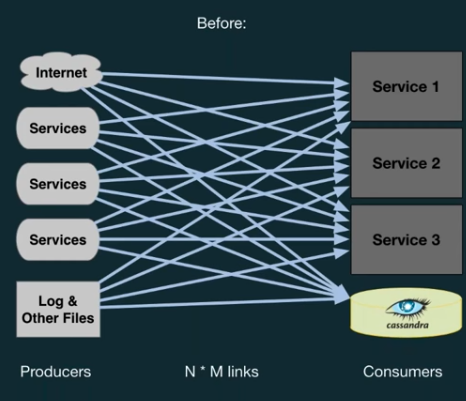
\includegraphics[width=5cm]{before-kafka}
	\caption{Create something like this for the actual components.}\label{fig:before-kafka}
\end{figure}

\begin{figure}
	\centering
	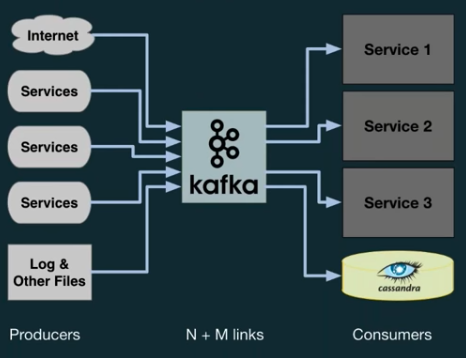
\includegraphics[width=5cm]{after-kafka}
	\caption{Create something like this for the actual components.}\label{fig:after-kafka}
\end{figure}



\section{Implementation}

\LaTeX{} and Bib\TeX{} style files, and Word templates that implement these 
instructions can be retrieved electronically.  See the ACRA homepage for 
details under
\verb+http://www.araa.asn.au/acra+

\subsection{Settings}

Prepare manuscripts two columns to a page, in the manner in which these
instructions are printed.  The exact dimensions for pages are:
\begin{itemize}
\item left and right margins: $.75''$
\item column width: $3.375''$
\item gap between columns: $.25''$
\item top margin---first page: $1.375''$
\item top margin---other pages: $.75''$
\item bottom margin: $1.25''$
\item column height---first page: $6.625''$
\item column height---other pages: $9''$
\end{itemize}

All measurements assume an {\bf $8$-$1/2 \times 11''$} page size.  
For A4-size paper use the given top and left margins, column width,
height, and gap and modify the bottom and right margins as necessary.

\subsection{Tracking State of the Agents}

Center the title on the entire width of the page in a 14-point bold font.
Place the names of authors below the title in a 12-point bold font, and
affiliations and complete addresses directly below the author names in a
12-point (non-bold) font.

Credit to a sponsoring agency appears in a footnote at the bottom of the
left column of the first page.  See the example in these instructions.

\subsection{Persistence}

Place the abstract at the beginning of the first column $3.0''$ from the
top of the page, unless that does not leave enough room for the title and
author information.  Use a slightly smaller width than in the body of the
paper.  Head the abstract with ``Abstract'' centered above the body of the
abstract in a 12-point bold font.  The body of the abstract should be in
the same font as the body of the paper.

The abstract should be a concise, one-paragraph summary
describing the general thesis and conclusion of your
paper. A reader should be able to learn the purpose of the
paper and the reason for its importance from the abstract. The
abstract should be no more than 200 words long.

\subsection{Visualization}

The main body of the text immediately follows the abstract. 
Use 10-point type in a clear, readable font with 1-point leading (10 on
11).  For reasons of uniformity, use Computer Modern font if possible.  If
Computer Modern is unavailable, Times Roman is preferred.

Indent when starting a new paragraph, except after major headings.

\subsection{Grid Search}

When necessary, headings should be used to separate major sections of your
paper.
(These instructions use many headings to demonstrate their
appearance---your paper should have fewer headings.)


\section{Agent Control a.k.a. (communication with) the Solver}

\section{Conclusions}

\section*{Acknowledgments}
The preparation of these instructions and the LaTEX and BibTEX files that implement them was supported by Schlumberger Palo Alto Research, AT\&T Bell Laboratories, and Morgan Kaufmann Publishers.


%% This section was initially prepared using BibTeX.  The .bbl file was
%% placed here later
%\bibliography{publications}
%\bibliographystyle{named}
%% The file named.bst is a bibliography style file for BibTeX 0.99c
\bibliographystyle{named}
\bibliography{bibfile}



\end{document}

